%% Problema: deve essere grassetto nella ToC e nel titolo del capitolo, ma non grassetto nell'header.
\chapter{Signal event selection}
\label{cap:event_selection}

\section{Prefiltering}
\label{sec:prefilter}
\textit{Prefilters}, also refered to as \textit{preliminary selections} or simply \textit{pre-selections}, are the foundation of the signal selection process.
The main objective of this step is to improve the signal-to-background ratio and reduce the computational workload to analyze data with cuts on kinematic variables.

\begin{table}[t]
	\begin{center}
	\begin{tabular}{@{}llll@{}}
		\toprule
		Variable & Unit & Minimum & Maximum \\
		\midrule
		$p(p)$ 						& MeV/$c$ 	& 2\,000	& 500\,000 \\
		$p_T(p)$ 					& MeV/$c$ 	& 400		& -- \\
		$p(\pi^-)$ 					& MeV/$c$ 	& 10\,000	& 500\,000 \\
		$z_\Lambda^\text{vtx}$		& mm		& 5\,500	& 8\,500 \\
		$p_T(\Lambda^0)$ 			& MeV/$c$ 	& 450		& -- \\
		$m(p\pi^-)$	(Vertex Fitter)	& MeV/$c^2$	& 600		& 1\,500 \\
		$m(p\pi^-)$	(combined)		& MeV/$c^2$	& --		& 2\,000 \\
		$m(p\pi^-)$	(measured)		& MeV/$c^2$	& --		& 1\,500 \\
		$\cos\xi_p (\Lambda^0)$		& --		& 0.9999	& -- \\
		$\Delta \chi^2_\text{PV} (\Lambda^0)$
									& -- 		& --		& 200 \\
		$\chi^2_\text{dist} (\Lambda^0)$
									& --		& --		& $2\times{10}^{7}$ \\
		$\chi^2_\text{vtx} (\Lambda^0)$
									& --		& --		& 750 \\
		$\lvert m(\mu^+ \mu^-) - m_\text{PDG} (J/\psi) \rvert$
									& MeV/$c^2$ & --		& 90 \\
		$m(J/\psi~\Lambda^0)$ (combined)
									& MeV/$c^2$	& 4\,700		& -- \\
		$m(J/\psi~\Lambda^0)$ (Vertex Fitter)
									& MeV/$c^2$	& --		& 8\,500 \\
		$\lvert \cos\xi_p (\Lambda^0_b) \rvert$
									& --		& 0.99		& -- \\
		$\Delta \chi^2_\text{PV} (\Lambda^0_b)$
									& -- 		& --		& 1\,750 \\
		$\chi^2_\text{vtx} (\Lambda^0_b)$
									& --		& --		& 150 \\
		\bottomrule
	\end{tabular}
	\end{center}
	\caption{Prefilter selection criteria applied to simulated \demonstratorshort signal and Run 2 data. The Vertex Fitter invariant mass is computed by the homonymous algorithm; the \textit{combined} invariant mass is computed from the 4-momenta of the daughter particles at the first measurement position, without track extrapolation; the \textit{measured} invariant mass is computed in the same way as the combined mass, but after extrapolation at the reconstructed decay vertex of the mother particle. Angle $\xi_p$ for a particle is computed between the line connecting its origin and decay vertices and the direction of its momentum. $\Delta \chi^2_\text{PV} (\Lambda^0)$ is the increase of the primary vertex $\chi^2$ when the particle is included in the fit. $\chi^2_\text{dist}$ is the geometrical distance between the primary vertex and the particle decay vertex in $\chi^2$ units.}
	\label{tab:4:prefilters}
\end{table}

\begin{figure}[t]
	\centering
	\begin{subfigure}{.45\textwidth}
		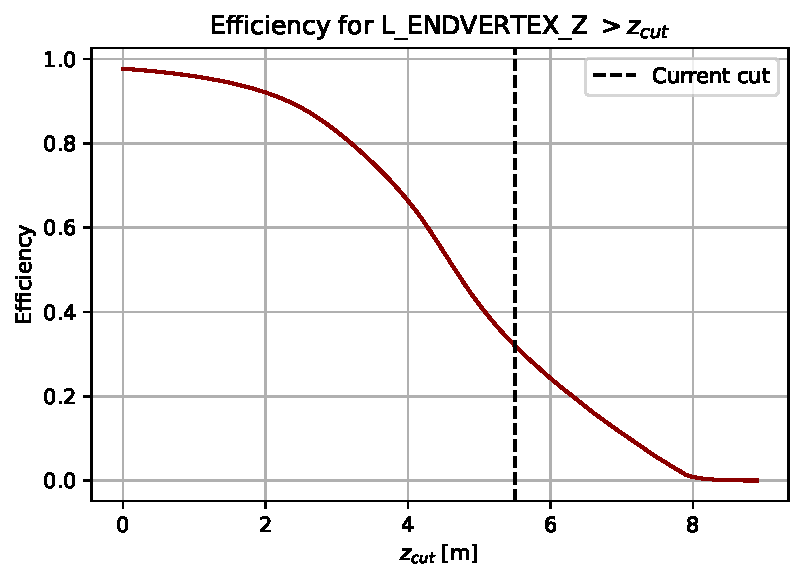
\includegraphics[width=\textwidth]{graphics/04-event_selection/LEVz_left.pdf}
		\caption{}
	\end{subfigure}
	\begin{subfigure}{.45\textwidth}
		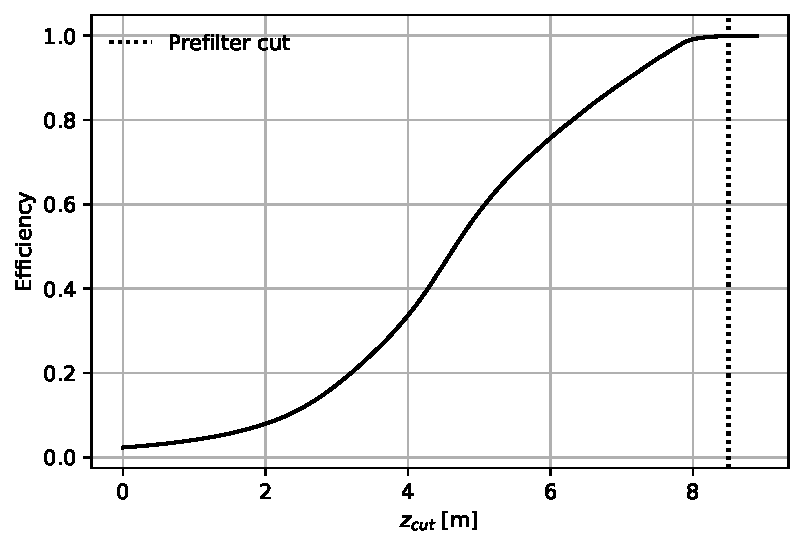
\includegraphics[width=\textwidth]{graphics/04-event_selection/LEVz_right.pdf}
		\caption{}
	\end{subfigure}
	\caption{Efficiency of the $z_\text{vtx}^\Lambda \geq z_\text{cut}^\text{left}$ \textit{(a)} and $z_\text{vtx}^\Lambda \leq z_\text{cut}^\text{right}$ \textit{(b)} prefilter selection criteria on \demonstratorshort simulated signal, as function of the respective thresholds. The \textit{dotted vertical lines} mark the chosen thresholds.}
	\label{fig:4:z_lambda_cuts}
\end{figure}

The applied prefilter criteria are listed in Table \ref{tab:4:prefilters}.
Efficiencies on signal have been estimated with studies on simulated \demonstratorshort events.
The most impactful selection is the one applied to $z_\text{vtx}^\Lambda$, the $z$ component of the \lambdadecay decay vertex;
the efficiencies for the left and right cuts as a function of the threshold are shown in Figure \ref{fig:4:z_lambda_cuts}.
Since I require $\Lambda^0$ to decay after the dipole magnet in order to observe spin precession, the [@todo] efficiency of the $z_\text{vtx}^\Lambda \geq \SI{5.5}{\meter}$ cut cannot be avoided.
Other selections have a much lower impact on signal, with efficiencies $\gtrsim 80\%$, resulting in a total prefilter efficiency of [@todo].

As detailed in Section \ref{sec:2:tracking}, a key aspect of my analysis is the employment of T tracks for the reconstruction of the \lz.
The low residual magnetic field for protons and pions produced far from the dipole magnet lowers momentum resolution for the associated tracks down to $20\% \div 30\%$.
Resolution can be improved up to $\approx 10\%$ by placing kinematic constraints on $p\pi^-$ and $\mu^+ \mu^-$ invariant masses, fixing them to the PDG values of $m(\Lambda^0)$ and $m(J/\psi)$ respectively (these will be henceforth referred to as \textit{mass constraints}).
This approach cannot be implemented in the leaf-by-leaf framework of the default Vertex Fitter algorithm for vertex reconstruction;
instead each event is refitted with the Decay Tree Fitter (DTF) algorithm in two configurations (single $J/\psi$ and double $J/\psi~\Lambda^0$ mass constraints (see also Section \ref{sec:3:dtf}).

A convergence requirement of the DTF algorithm with the $J/\psi~\Lambda^0$ mass constraints is therefore added to the prefilter selections.
The main drawback of this selection, a much steeper [@todo] efficiency on simulated signal events, is outweighed by the benefits of the improved momentum resolution in the determination of the angular distribution of \lambdadecay decay products.


\subsection{Reconstruction of \texorpdfstring{\lz}{Lambda} decay vertex in prefiltered events}
\label{sec:lambda_endvertex_bias}

The quality of the \lambdadecay vertex reconstruction affects many aspects of the $\Lambda^0$ electromagnetic dipole moments measurement:
on top of being fundamental to evaluate how much magnetic field the particle traversed (and thus the extent of spin precession), even the best momentum resolution for protons and pions is worthless if the particles are extrapolated at the wrong point of production.
Both $x_\text{vtx}^\Lambda$ and $y_\text{vtx}^\Lambda$ are fairly well reconstructed in prefiltered events, with resolution $\lesssim \SI{1}{\centi\meter}$ and no discernible bias.
This section will therefore focus on the reconstruction of $z_\text{vtx}^\Lambda$.

\begin{figure}[t]
	\centering
	\begin{subfigure}{.45\textwidth}
		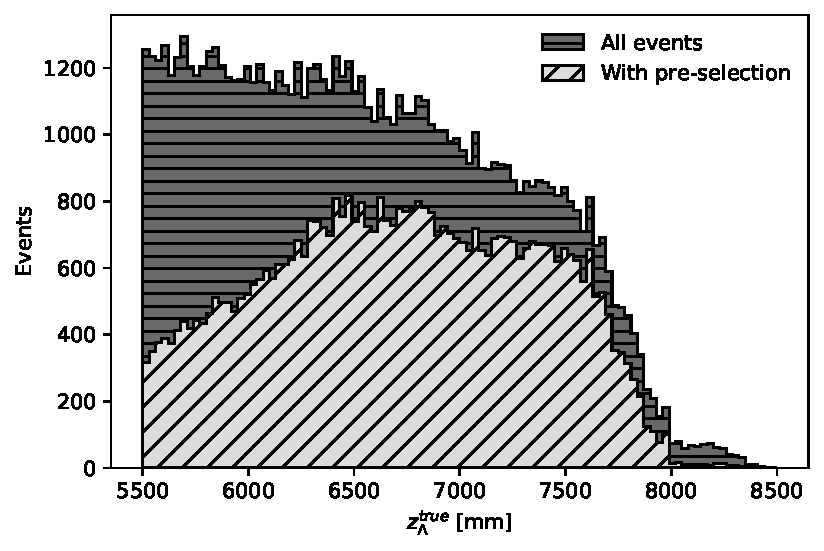
\includegraphics[width=\textwidth]{graphics/04-event_selection/Lambda_endvertex_z_true.pdf}
		\caption{}
		\label{fig:4:lz_vertex_true}
	\end{subfigure}
	\begin{subfigure}{.45\textwidth}
		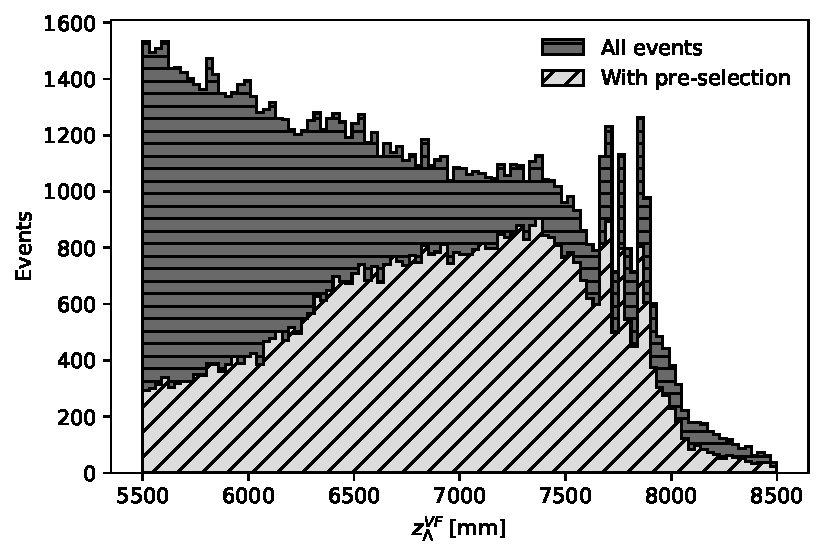
\includegraphics[width=\textwidth]{graphics/04-event_selection/Lambda_endvertex_z.pdf}
		\caption{}
		\label{fig:4:lz_vertex_reco}
	\end{subfigure}
	\caption{Distribution of true \textit{(a)} and reconstructed \textit{(b)} $z_\text{vtx}^\Lambda$ in simulated \demonstratorshort signal events, without (\textit{dark grey}) and with (\textit{light grey}) prefiltering.}
	\label{fig:4:lz_vertex_distributions}
\end{figure}

\begin{figure}[t]
	\centering
	\begin{subfigure}{.45\textwidth}
		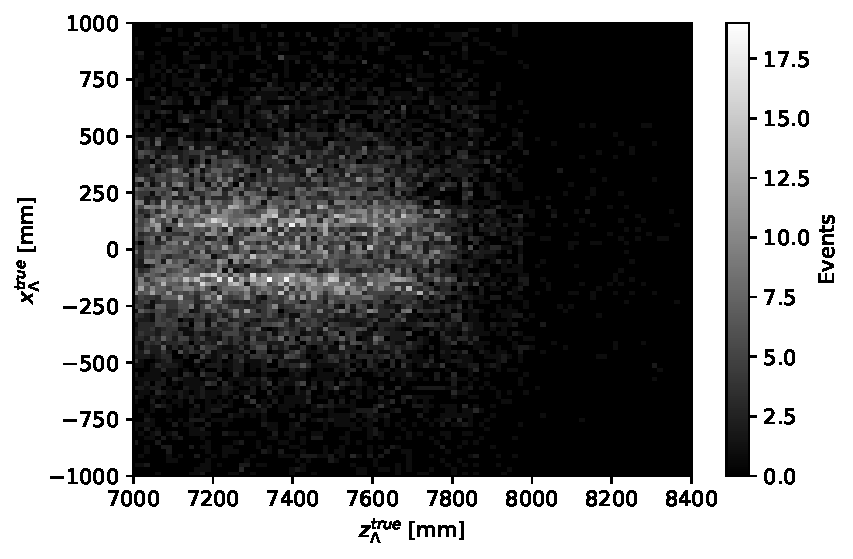
\includegraphics[height=.2\textheight]{graphics/04-event_selection/Lambda_endvertex_z_vs_x_true.pdf}
		\caption{}
		\label{fig:4:lz_vertex_peaks_true}
	\end{subfigure}
	\begin{subfigure}{.45\textwidth}
		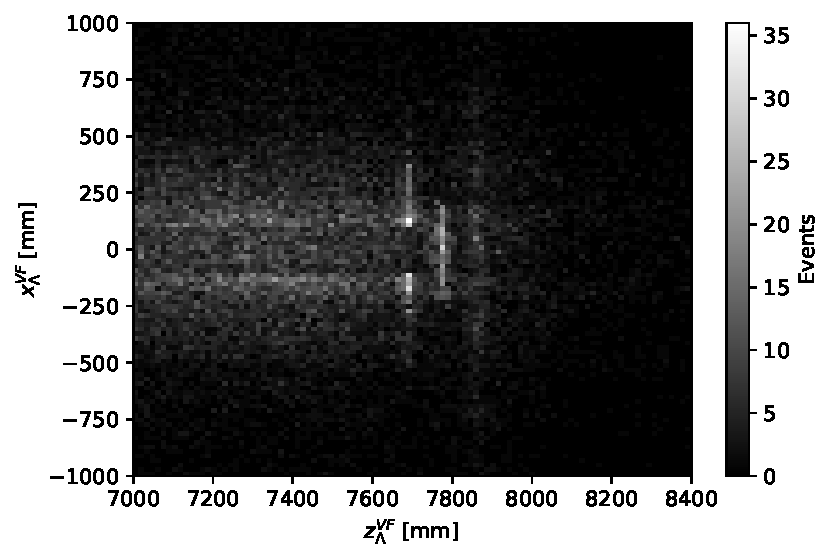
\includegraphics[height=.2\textheight]{graphics/04-event_selection/Lambda_endvertex_z_vs_x.pdf}
		\caption{}
		\label{fig:4:lz_vertex_peaks_reco}
	\end{subfigure}
	\caption{Distribution of simulated \demonstratorshort signal events (prefilters applied) with $z_\Lambda^\text{VF} \geq \SI{7.0}{\meter}$, as function of true (\textit{left}) and reconstructed (\textit{right}) $x_\Lambda^\text{vtx}$ and $z_\text{vtx}^\Lambda$. This corresponds to a top view of true and reconstructed \lz decay vertices.}
	\label{fig:4:lz_vertex_peaks}
\end{figure}

Figures \ref{fig:4:lz_vertex_true} and \ref{fig:4:lz_vertex_reco} show the distributions of true and reconstructed $z_\text{vtx}^\Lambda$ respectively for simulated signal events.
The most prominent difference between the two is the presence of three peaks in the $[\SI{7.5}{\meter},\SI{8.0}{\meter}]$ region of the reconstructed distribution, being found both with and without prefilter selections. 
The significance of these structures can be inferred by plotting the events as function of  $z_\text{vtx}^\Lambda$ and $x_\text{vtx}^\Lambda$, corresponding to a bending plane perspective of the detector.
This is shown in Figure \ref{fig:4:lz_vertex_peaks_reco}, highlighting the fact that the peaks in $\Lambda^0$ decay vertices have a very precise geometrical location, absent when comparing the true $z_\text{vtx}^\Lambda$ and $x_\text{vtx}^\Lambda$ values for the same events (Figure \ref{fig:4:lz_vertex_peaks_true}).
The spatial distribution of the vertices bears a striking resemblance to the layout of a T tracking station (see Figure \ref{fig:2:t_station_top}) and $z$ coordinates are consistent with the nominal placement of IT and first OT plane of the T1 station \cite{Barbosa-Marinho:582793}.
While dedicated studies are required to gain more insight into the source of these structures, they are assumed to be of minor impact for the purposes of this thesis.

\begin{figure}[t]
	\centering
	\begin{subfigure}{.45\textwidth}
		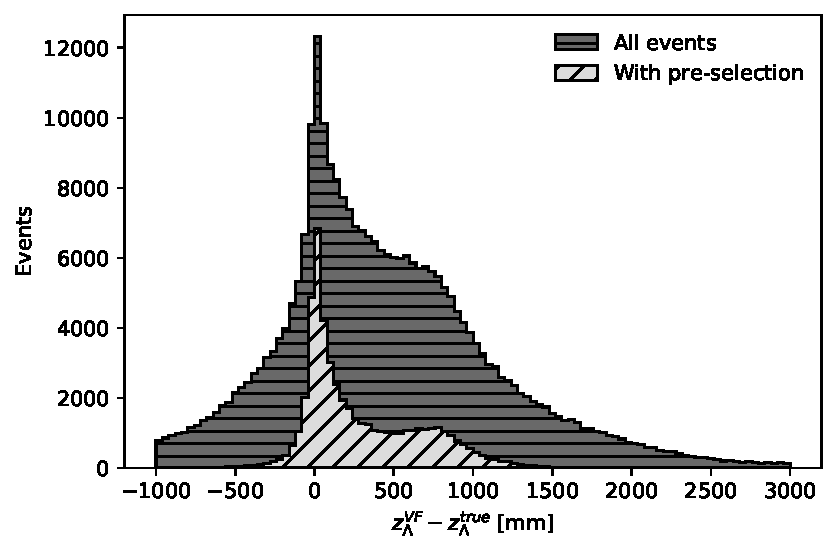
\includegraphics[width=\textwidth]{graphics/04-event_selection/Lambda_endvertex_bias_z.pdf}
		\caption{}
	\end{subfigure}
	\begin{subfigure}{.45\textwidth}
		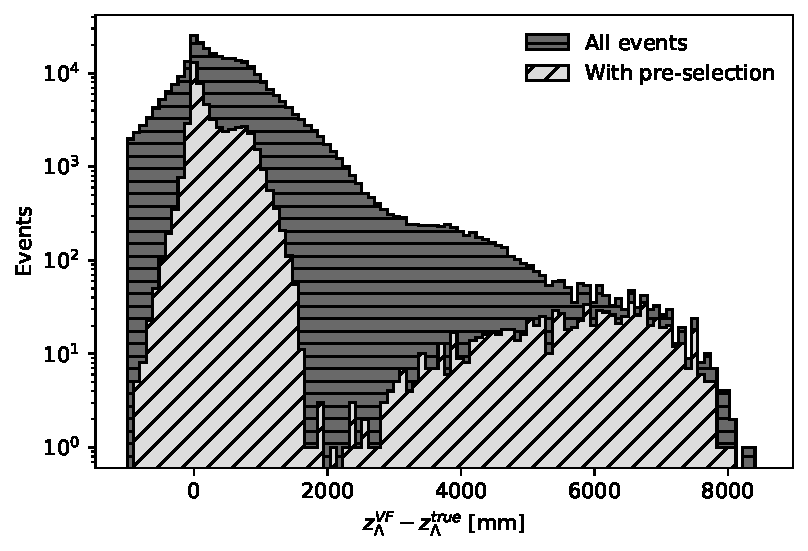
\includegraphics[width=\textwidth]{graphics/04-event_selection/Lambda_endvertex_bias_z_log.pdf}
		\caption{}
	\end{subfigure}
	\caption{Distribution of $z_\text{vtx}^\Lambda$ bias for simulated \demonstratorshort events in linear \textit{(a)} and logarithmic \textit{(b)} scales, without (\textit{dark grey}) and with (\textit{light grey}) prefiltering.}
\end{figure}

The differing shapes of true and reconstructed $z_\text{vtx}^\Lambda$ distributions from Figure \ref{fig:4:lz_vertex_distributions} are also evidence of bias effects in the \lambdadecay vertex reconstruction.

\begin{figure}[t]
	\centering
	\begin{subfigure}{.45\textwidth}
		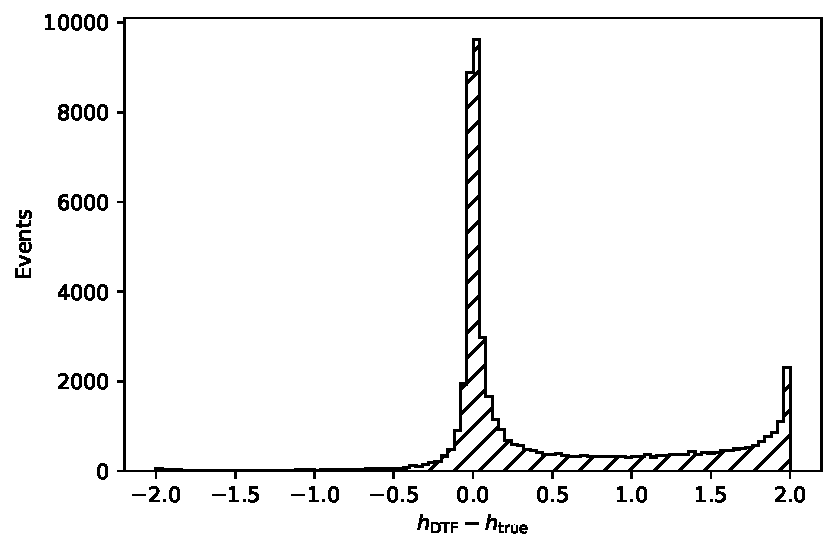
\includegraphics[width=\textwidth]{graphics/04-event_selection/Lambda_horizontality_bias.pdf}
		\caption{}
	\end{subfigure}
	\begin{subfigure}{.45\textwidth}
		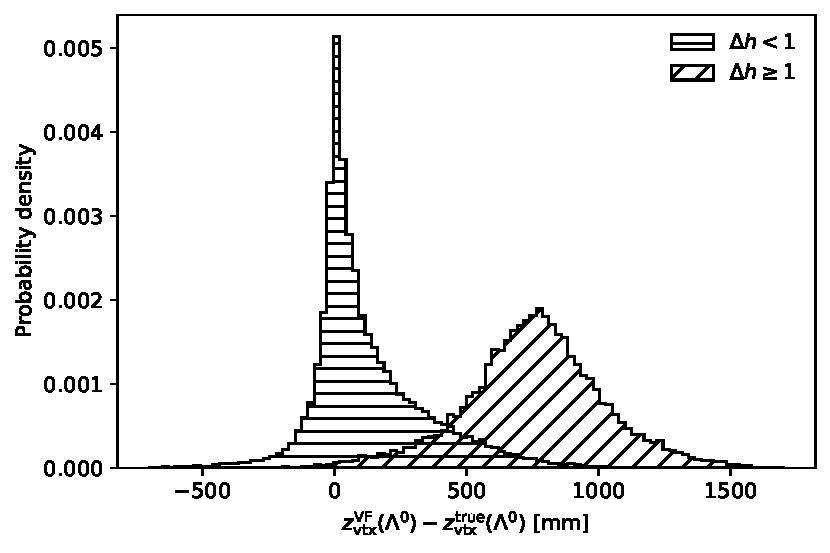
\includegraphics[width=\textwidth]{graphics/04-event_selection/lambda_endvertex_z_bias_vs_horizontality_bias.pdf}
		\caption{}
	\end{subfigure}
	\caption{\textit{(a)} Horizontality bias distribution for simulated \demonstratorshort events (prefilters applied), comparing results from Decay Tree Fitter algorithm with \jpsi and \lz mass constraints with true values. \textit{(b)} Distribution of $z_\text{vtx}^\Lambda$ bias for events with horizontality bias $<1$ (\textit{horizontal hatching}) and $\geq 1$ (\textit{diagonal hatching}).}
\end{figure}

\begin{figure}[t]
	\centering
	\begin{subfigure}{.45\textwidth}
		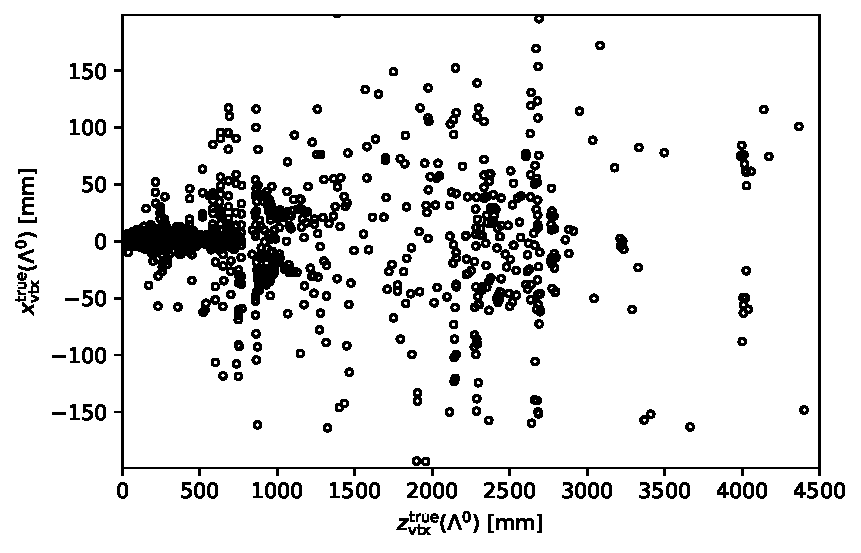
\includegraphics[width=\textwidth]{graphics/04-event_selection/bump_Lambda_true_endvertex_z_vs_x.pdf}
		\caption{}
	\end{subfigure}
	\begin{subfigure}{.45\textwidth}
		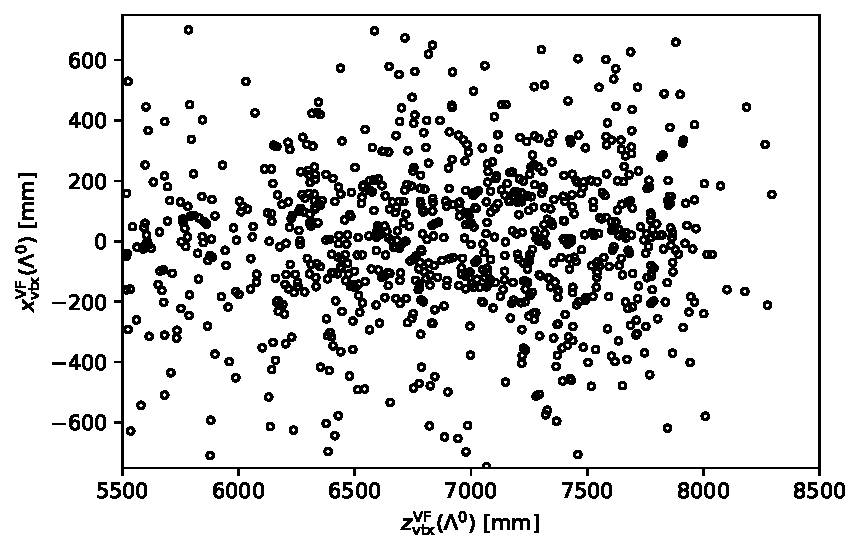
\includegraphics[width=\textwidth]{graphics/04-event_selection/bump_scatter_Lambda_endvertex_z_vs_x.pdf}
		\caption{}
	\end{subfigure}
	\caption{Distribution of simulated \demonstratorshort events (prefilters applied) with $z_\Lambda^\text{VF} - z_\Lambda^\text{true} \geq \SI{2.0}{\meter}$ as function of true \textit{(a)} and reconstructed \textit{(b)} $x_\Lambda^\text{vtx}$ and $z_\text{vtx}^\Lambda$. This corresponds to a top view of true and reconstructed \lz decay vertices.}
\end{figure}

Qui devi menzionare l'orizzontalità, perché vi faccio riferimento nel Cap. 3. Devi dire che c'è il problema con grafico. Aggiungi il diagramma che spiega cos'è, quello con h=+-1, 0.

\section{Physical background veto}
\label{sec:B0_veto}
\begin{figure}[t]
	\centering
	\begin{subfigure}{.45\textwidth}
		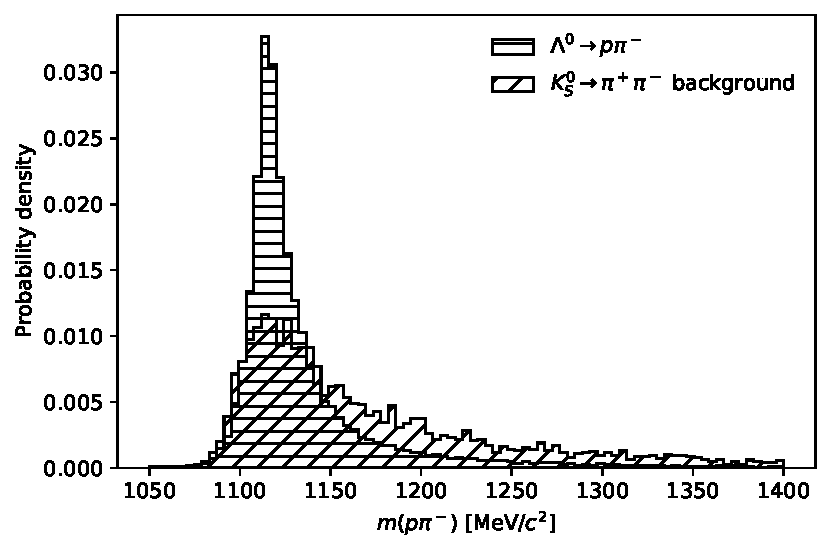
\includegraphics[width=\textwidth]{graphics/04-event_selection/phys_bkg_lambda_comparison.pdf}
		\caption{}
	\end{subfigure}
	\begin{subfigure}{.45\textwidth}
		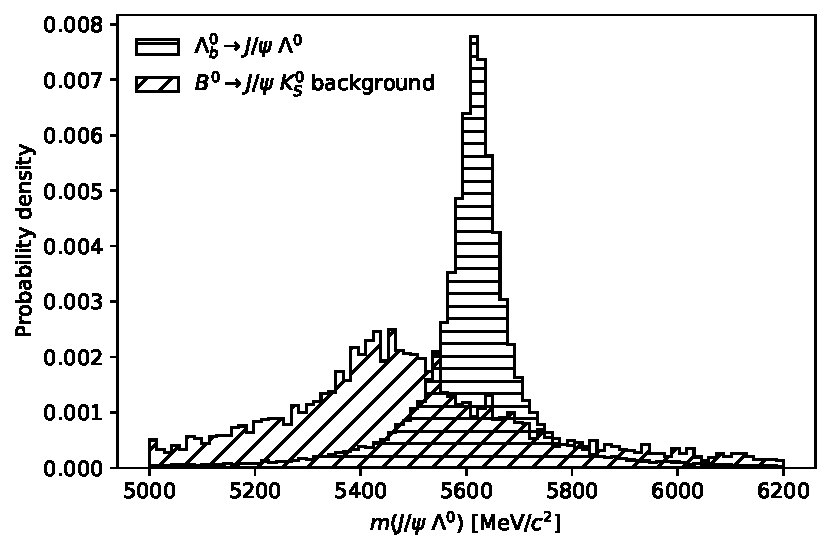
\includegraphics[width=\textwidth]{graphics/04-event_selection/phys_bkg_lambdab_comparison.pdf}
		\caption{}
	\end{subfigure}
	\caption{Comparison of simulated $m(p\pi^-)$ \textit{(a)} and $m(J/\psi~\Lambda^0)$ \textit{(b)} distributions: \demonstratorshort signal is labeled by \textit{horizontal hatching}, \physbkgshort physical background with $\pi^+ \rightarrow p$ mass hypothesis by \textit{diagonal hatching}.}
\end{figure}

\begin{figure}[t]
	\centering
	\begin{subfigure}{.45\textwidth}
		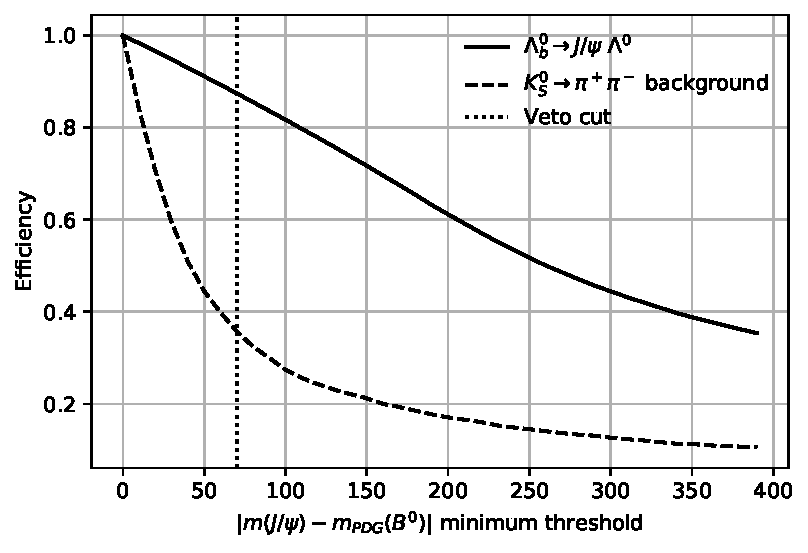
\includegraphics[height=.2\textheight]{graphics/04-event_selection/phys_veto_efficiencies.pdf}
		\caption{}
	\end{subfigure}
	\begin{subfigure}{.45\textwidth}
		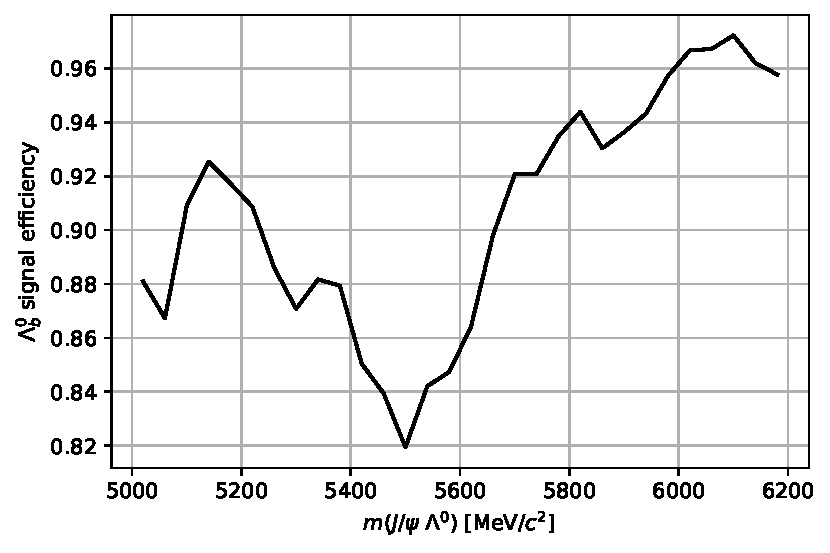
\includegraphics[height=.2\textheight]{graphics/04-event_selection/phys_veto_sig_efficiencies_per_bin.pdf}
		\caption{}
	\end{subfigure}
	\caption[Efficiency of the physical background veto as a function of the invariant mass discrepancy threshold and of $J/\psi~\Lambda^0$ invariant mass bins.]{\textit{(a)} Efficiency of physical background veto as a function of the invariant mass discrepancy threshold on simulated signal (\demonstratorshort, solid) and background (\physbkgshort with proton mass hypothesis, dashed) events. Chosen threshold marked by dotted line. \textit{(b)} Efficiency of the veto on different $m(J/\psi~\Lambda^0)$ bins for \demonstratorshort signal events).}
\end{figure}

\section{HBDT classifier}
\label{sec:HBDT}

\subsection{Training data}

\begin{figure}[t]
	\centering
	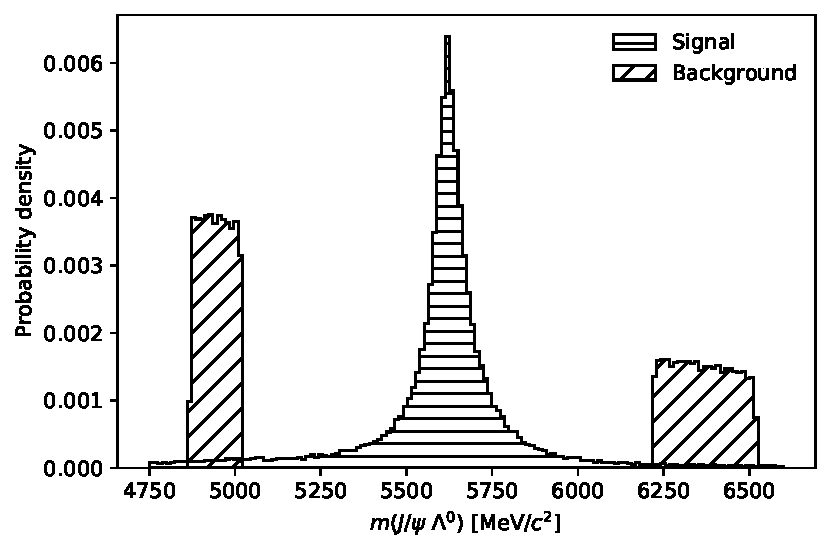
\includegraphics[width=.6\textwidth]{graphics/04-event_selection/sig_bkg_distribution_balance.pdf}
	\caption{Signal (\textit{horizontal hatching}) and background (\textit{diagonal hatching}) data samples used for training the HBDT classifier. Test samples are taken from the same pool in 1:9 ratio.}
	\label{fig:4:HBDT_training_data}
\end{figure}

\subsection{Hyperparameter optimization and performance test}
\begin{figure}[t]
	\centering
	\begin{subfigure}{.45\textwidth}
		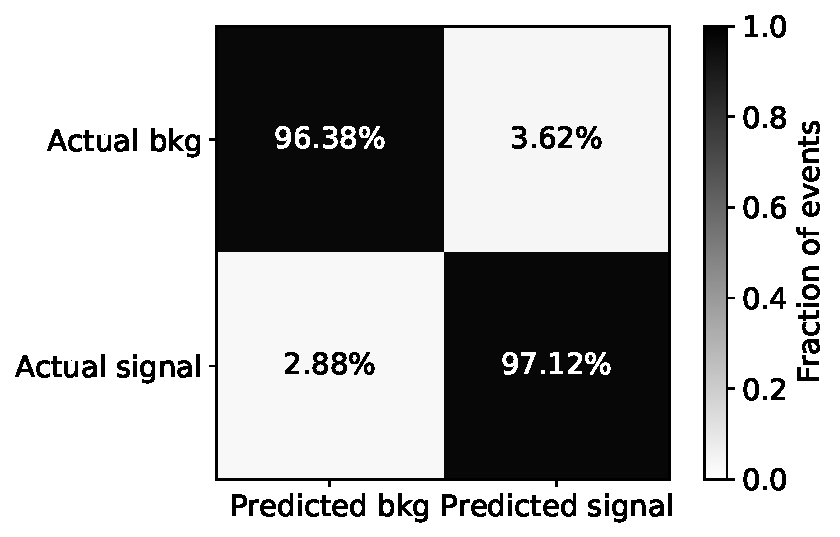
\includegraphics[width=\textwidth]{graphics/04-event_selection/confmatrix_train.pdf}
		\caption{}
	\end{subfigure}
	\begin{subfigure}{.45\textwidth}
		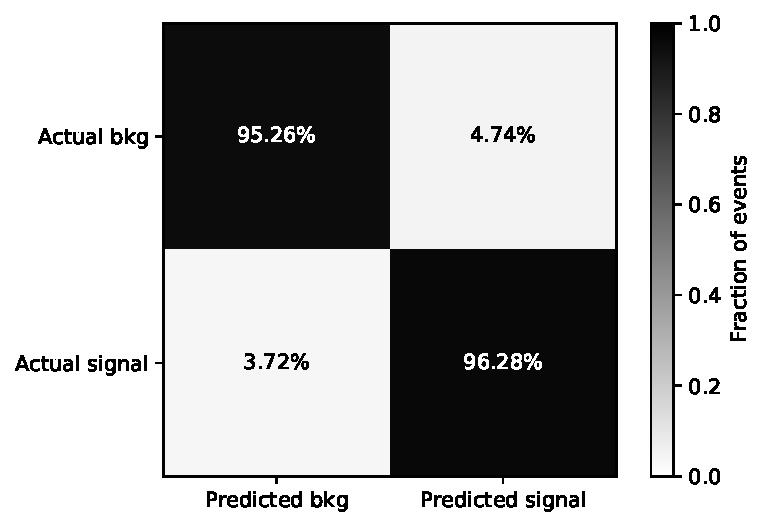
\includegraphics[width=\textwidth]{graphics/04-event_selection/confmatrix_test.pdf}
		\caption{}
	\end{subfigure}
	\caption{Confusion matrices visualizing the performance of the HBDT classifier on training \textit{(a)} and testing \textit{(b)} data samples. Percentages and chromatic scale are normalized to the true event classification: for instance, the top left and top right quadrants of a matrix represent the fraction of true background events reconstructed as background or signal, respectively. Binary classification uses an illustrative response threshold $s_\text{thres} = 0.5$.}
\end{figure}

\begin{figure}[t]
	\centering
	\begin{subfigure}{.45\textwidth}
		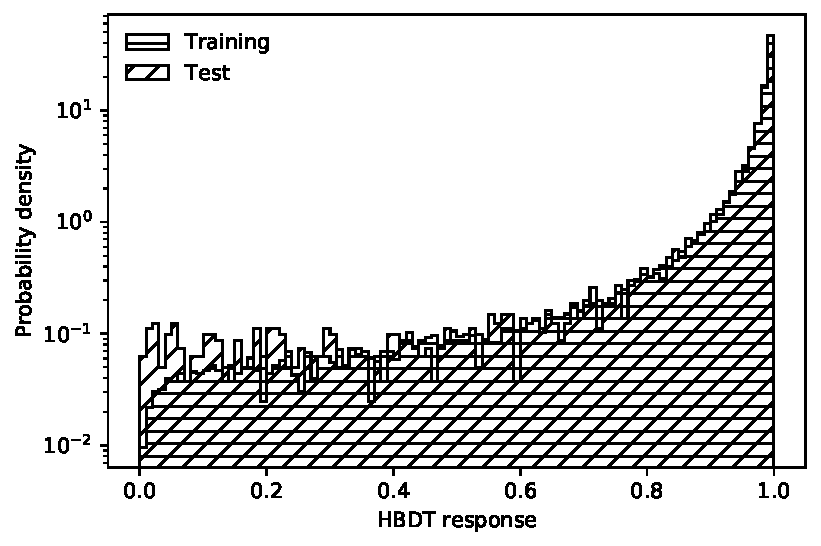
\includegraphics[width=\textwidth]{graphics/04-event_selection/sig_train_vs_test.pdf}
		\caption{}
	\end{subfigure}
	\begin{subfigure}{.45\textwidth}
		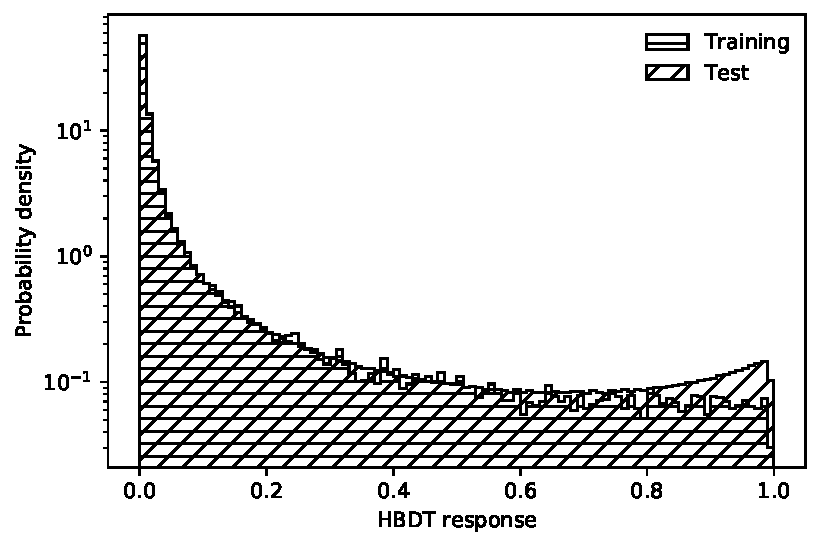
\includegraphics[width=\textwidth]{graphics/04-event_selection/bkg_train_vs_test.pdf}
		\caption{}
	\end{subfigure}
	\caption{Response distribution of the HBDT classifier on signal \textit{(a)} and background \textit{(b)} events. The training sample is represented by horizontal hatching, the test sample by diagonal hatching.}
\end{figure}

\begin{figure}
	\centering
	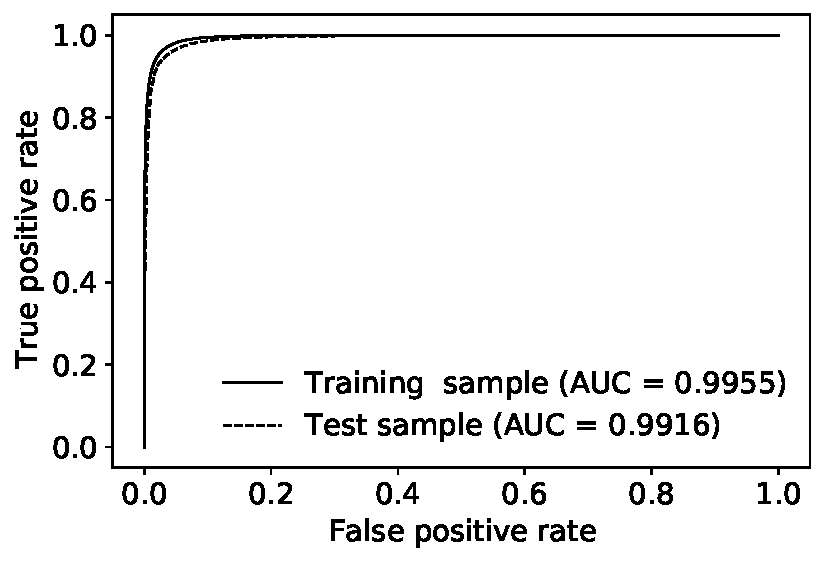
\includegraphics[width=.6\textwidth]{graphics/04-event_selection/roc.pdf}
	\caption{Receiving operating characteristic (ROC) curve for the HBDT classifier on training (\textit{solid}) and test (\textit{dashed}) samples. The legend includes the area-under-curve (AUC) score.}
\end{figure}

\subsection{Threshold optimization}

\begin{figure}
	\centering
	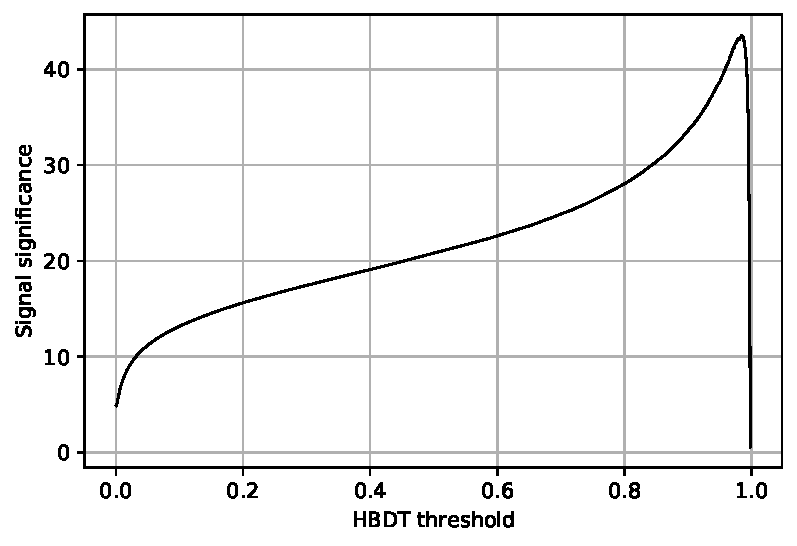
\includegraphics[width=.6\textwidth]{graphics/04-event_selection/HBDT_signal_significance.pdf}
	\caption{Projected \demonstratorshort signal significance over background as a function of the HBDT response threshold used for selection.}
\end{figure}

\section{Performance on data}
Gli invariant mass fits, essenzialmente.

\begin{figure}[t]
	\centering
	\begin{subfigure}{.45\textwidth}
		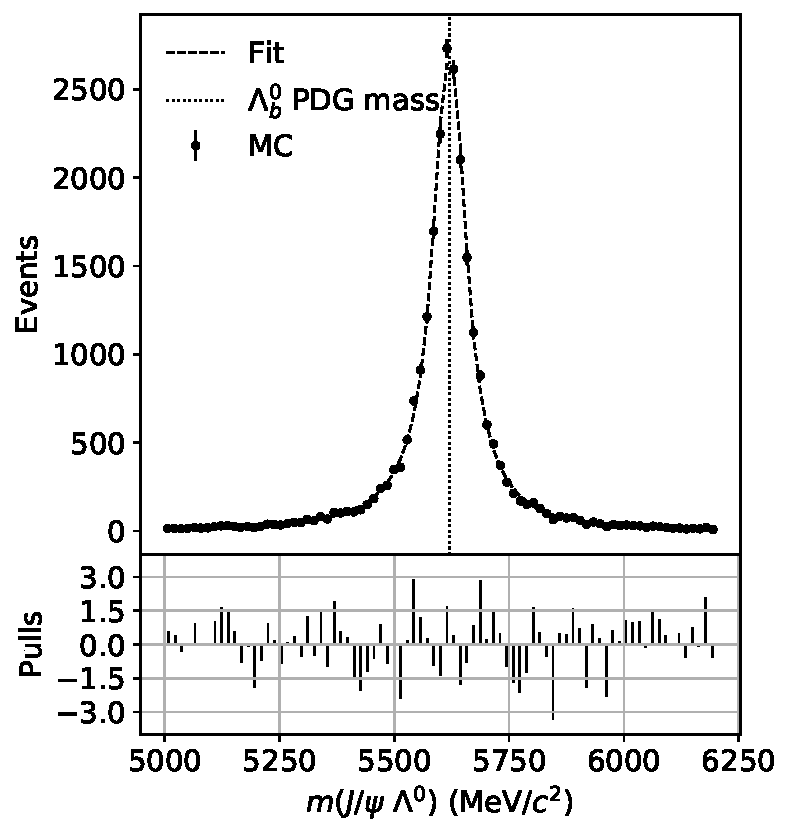
\includegraphics[width=\textwidth]{graphics/04-event_selection/MC_lambdab_hard_fit.pdf}
		\caption{}
	\end{subfigure}
	\begin{subfigure}{.45\textwidth}
		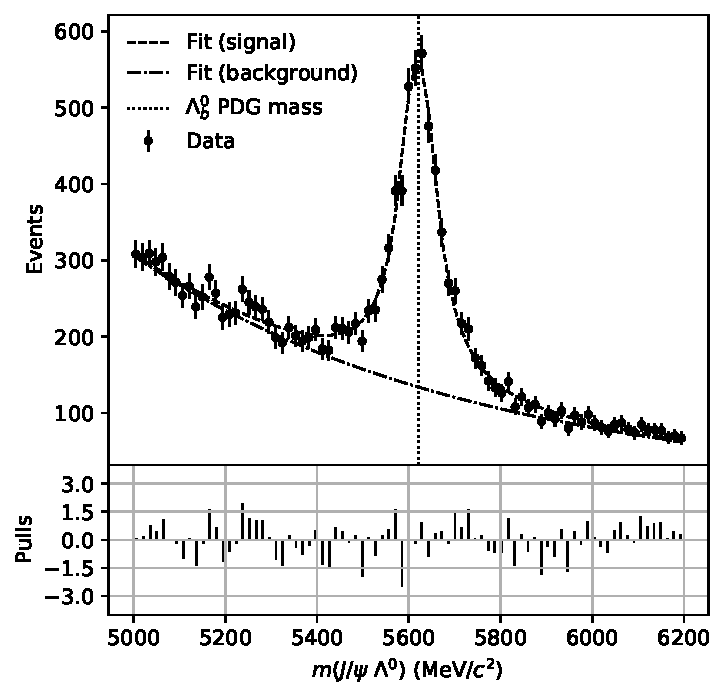
\includegraphics[width=\textwidth]{graphics/04-event_selection/data_lambdab_hard_fit.pdf}
		\caption{}
	\end{subfigure}
	\caption{Fitted $m(J/\psi~\Lambda^0)$ invariant mass distributions for simulated \demonstratorshort events \textit{(a)} and Run 2 data \textit{(b)} after all selection steps. Signal fit function is \textit{dashed}, background fit function in \textit{(b)} is \textit{dash-dotted}. The current best measurement for $\Lambda_b^0$ mass is marked by the \textit{dotted vertical line}. Fit pulls (data-fit discrepancy divided by uncertainty) are shown below the main plots.}
\end{figure}
